%%%%%%%%%%%%%%%%%%%%%%%%%%%%%%%%%%%%%%%%%%%%%%%%%%%%%%%%%%%%%%%%%%%%%%%%%%%%%%%%%%%%%%%%%%%%%%%
%Plantilla: para la realizaci�n de informes.
%Curso:     Simulaci�n estad�stica.
%Profesor:  Johann A. Ospina.
%%%%%%%%%%%%%%%%%%%%%%%%%%%%%%%%%%%%%%%%%%%%%%%%%%%%%%%%%%%%%%%%%%%%%%%%%%%%%%%%%%%%%%%%%%%%%%%


%Establece el tipo de documento (art�culo), tama�o de letra (10pt) a una columna.
\documentclass[letterpaper,12pt,onecolumn,titlepage]{article} 
 
 
% Cargar paquetes
\usepackage{verbatim}
\usepackage{mathrsfs}
\usepackage{amsmath}
\usepackage{amssymb}
\usepackage{subfigure}
\usepackage{ucs}
\usepackage[latin1]{inputenc}
\usepackage[spanish]{babel}
\usepackage{fontenc}
\usepackage{graphicx}
\usepackage{anysize}
\usepackage{fancyhdr}
\usepackage[comma,authoryear]{natbib}
\usepackage{url} %paquete para definir url
\usepackage{hyperref}  %hipervinculos

%Estilo de la p�gina
\pagestyle{fancy}

%Establecer el margen
\marginsize{2cm}{2cm}{1cm}{1cm}
\setlength{\headheight}{13.1pt}


% Portada
\title{
    \textbf{Laboratorio N.1}\
    ~\\{Introduccion a Los Metodos Estadisticos}   
    ~\\{Estimadores}}
\author{
    {Diana Carolina Arias Sinisterra Cod. 1528008}
 ~\\{Kevin Steven Chica Garcia Cod. 1533173}
 ~\\{Cesar Andres Saavedra Vanegas Cod. 1628466}}

\date{
     \textbf{Universidad Del Valle}\   
    ~\\{Facultad De Ingenieria}
    ~\\{Estadistica}
    ~\\{Octubre}
    ~\\{2017}}
 
 
 
\decimalpoint %Poner punto decimal
 
\begin{document}
 
% Se aplica el formato a las p�ginas. Se despliegan: portada e �ndices de materias, figuras y tablas
\renewcommand{\listtablename}{Indice de tablas}
\renewcommand{\tablename}{Tabla}
\maketitle
\setcounter{page}{2}
\tableofcontents{}
%\thispagestyle{empty}
%\newpage
\listoffigures{}
\listoftables

\thispagestyle{empty}

\newpage
\fancyhead{}
\fancyfoot{}
 
% Encabezado y pie de pagina
\lhead{Introduccion a los Metodos Estadisticos}
\lfoot{Universidad Del Valle}
\rfoot{\thepage}

% Estilo de la bibliograf�a
\bibliographystyle{apalike}
 
% Desarrollo de los contenidos del documento
\section{Situacion 1}

Despliegue de una tabla que se llama ``Tabla1'' junto a su n�mero de referencia:

\begin{table}[!h]
\centering
\caption{Titulo de la tabla}
\begin{tabular}{lrr}
\hline
{\bf Indicador} &  {\bf $\mathbf{SO_{2}}$} & {\bf Temperatura} \\
\hline
  Promedio &     0.006 &     24.093 \\

Desviaci�n est�ndar &     0.007 &       2.950 \\

   Mediana &     0.004 &       23.500 \\

    Minima &    0.000 &       18.200 \\

    M�ximo &     0.127 &         32 \\

 Asimetr�a &     5.415 &      0.451 \\
\hline
\end{tabular}
\label{tbl:Descriptivas}  
\end{table}

Para referenciar una tabla, se utiliza el texto ``ref'' precedido de un \textit{backslash}: as�, se referenciar�a la Tabla \ref{tbl:Descriptivas}.
\\
\\
Despliegue de una imagen que se llama ``Figura1'' junto a su n�mero de referencia:
 
\begin{figure}[!h]
    \begin{center}
        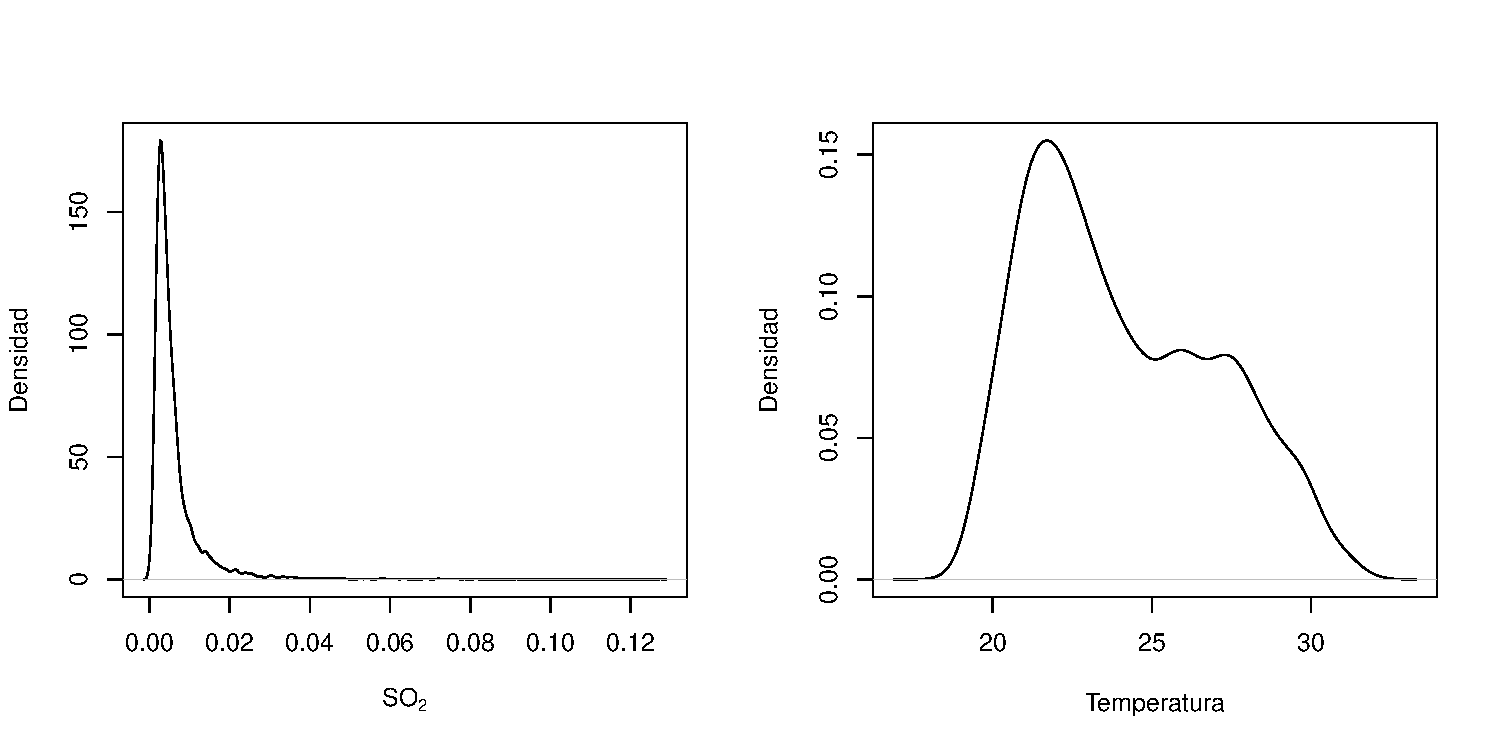
\includegraphics[width=10cm]{Figuras/Figura1.pdf}
        \caption{Titulo de la figura}
        \label{fig:Densidad}
    \end{center}
\end{figure}
 
Para referenciar una figura, se utiliza el texto ``ref'' precedido de un \textit{backslash}: as�, se referenciar�a la Figura \ref{fig:Densidad}.
\\
\\
Expresi�n matem�tica en l�nea con el texto: $f(x):=ax^2+bx+c$.
\\
\\ 
Representaci�n de una ecuaci�n, sin n�mero de referencia:
 
$$y_{i} = \beta_{0} + \beta_{1}x_{i} + \epsilon_{i}$$
 
Representaci�n de una ecuaci�n en una l�nea nueva, con n�mero de referencia:
 
\begin{equation}
 \bar{X} = \sum_{i=1}^{n}\frac{x_{i}}{n}
 \label{eq:media}
\end{equation}
 
Pare referenciar la ecuaci�n \eqref{eq:media}. Se utiliza la etiqueta ``eqref'' precedido de un \textit{backslash}
\\
\\
Para referenciar una cita bibliogr�ficas se utiliza un archivo ``Bibliografia.bib''. Este contiene la informaci�n de las referencias utilizadas. Por ejemplo para citar dentro del texto: Seg�n \cite{seber2012linear} plantea que el modelo de regresi�n.....

\subsection{}
 
$\left(\frac{365}{3}\right) \cdot \left(\frac{365}{4}\right) $
 
Una lista: 
 
\begin{itemize}
 \item primer �tem de la lista.
 \item segundo �tem de la lista.
\end{itemize}
 
Numeraci�n de una lista:
 
\begin{enumerate}
\item primer �tem de la lista.
\item segundo �tem de la lista.
\end{enumerate}


 
Ejemplo para construir una matriz:
 
$$I = \left[
\begin{array}{c c c c c}
        1    &    0    &    0    &    0    \\
        0    &    1    &    0    &    0    \\
        0    &    0    &    1    &    0    \\
        0    &    0    &    0    &    1
\end{array} \right]$$
 
% Insertar una gran cantidad de comentarios (bloque)
\begin{comment}
Este texto, al igual que aquel que est� precedido por un signo de porcentaje, no ser� mostrado en el documento final.
\end{comment}

\subsection{Scripts R}
El ambiente \emph{Verbatim} permite agregar codigo de R.
\begin{verbatim}
getwd()
k=70
cumpledif=1
p=0
q=0
for (j in 1:k){
  cumpledif=cumpledif*(1-((j-1)/365))
  q[j]=cumpledif
  p[j]=1-cumpledif
  cat(cumpledif,"\n")
}

windows()
pdf("Texmaker/Graficos/Punto2.pdf")
par(mfrow=c(1,3))
plot(p,col="red", xlab = "n", ylab = "Probabilidad", main = "Probabilidad de que dos o mas estudiantes 
tengan el mismo cumplea�os en funcion 
     de la cantidad de estudiantes n")
abline(h=0.5)
abline(v=23)

plot(q,col="blue", xlab = "n", ylab = "Probabilidad", main = "Probabilidad de que dos o mas estudiantes 
NO tengan el mismo cumplea�os en funcion 
     de la cantidad de estudiantes n")
abline(h=0.5)
abline(v=23)

plot(p,col="red", xlab = "", ylab = "")
par(new=TRUE)
plot(q,col="blue", xlab = "", ylab = "")

title(xlab = "n", ylab = "Probabilidad",main="Probabilidades de que dos o mas estudiantes 
tengan el mismo cumplea�os (rojo) y su 
evento complemetario (azul) en funcion de n")
dev.off()

###########simulacion punto 3a Exponencial

U = runif(1000, 0, 1) #Generar U
l = 4 #Par�ametro de la exponencial Lambda = 4
X = -(1/l) * log(U)
windows()
pdf("Texmaker/Graficos/Punto3A.pdf")
par(mfrow=c(1,2))
plot(density(U),col="blue", xlab = "X", ylab = "Densidad", main = expression(Unif(0,1)))
plot(density(X),col="red", xlab = "X", ylab = "Densidad", main = expression(Exp(lambda=4)))
dev.off()

############ Punto 3b Poisson 
x=0
for(j in 1:1000){
  lambda=7
  i = 0
  p = exp(-lambda)
  f = p
  u= runif(1000,0,1)
  while(u>=f){
    p=lambda*p/(i + 1)
    f = f + p
    i = i +1
    x[j] = i
  } 
}

\end{verbatim}


\subsection{Analisis Resultados}
\section{Situacion 1}
~\\ Los estimadores propuestos son:
~\ $$\hat{\theta_1}=2\bar{X}-1$$
~\ $$\hat{\theta_2}=X_{Max}+X_{Min}-1$$
~\ $$\hat{\theta_3}=X_{Max}$$
~\ $$\hat{\theta_4}=Me(X) $$
~\\ Para evaluar los estimadores anteriores obtuvimos las siguientes cuatro graficas:
\begin{figure}[!h]
    \begin{center}
        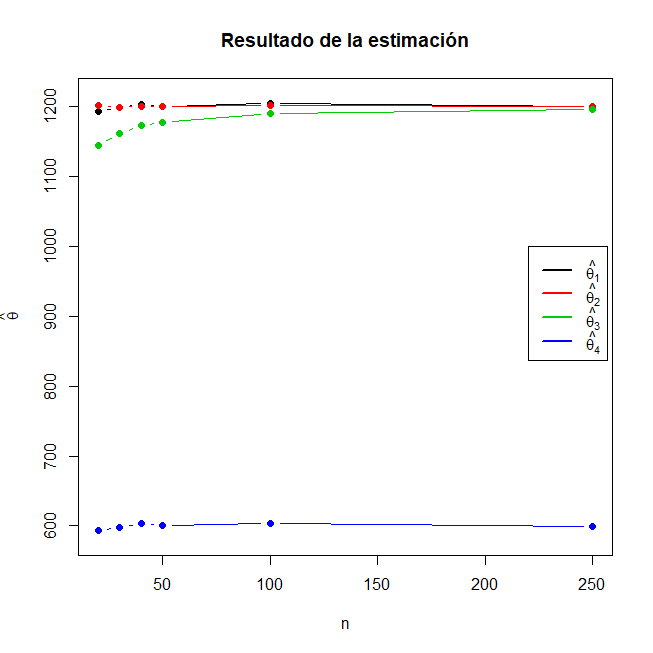
\includegraphics[width=10cm]{Figuras/A.png}
        \caption{Grafica del resultado de la estimacion del parametro real $\theta=1200$}
        \label{fig:Densidad}
    \end{center}
\end{figure}
~\\ Como podemos observar en la grafica,los estimadores $\hat{\theta_1}$ y $\hat{\theta_2}$ son los que mas se acercan al parametro real $\theta=1200$  con cualquier tama\~{n}o de muestra, aunque el estimador $\hat{\theta_3}$ tambien se acerca pero despues de tama\~{n}o de muestra $n=100$, lo cual nos dice que son mejores los dos anteriores. El estimador $\hat{\theta_4}$ esta muy lejos del parametro real, a simple vista podriamos decir que ese estimador serviria no para estimar $\theta$ en si, si no, para estimar la media de la distribucion en general que es aproximadamente 600.
\begin{figure}[!h]
    \begin{center}
        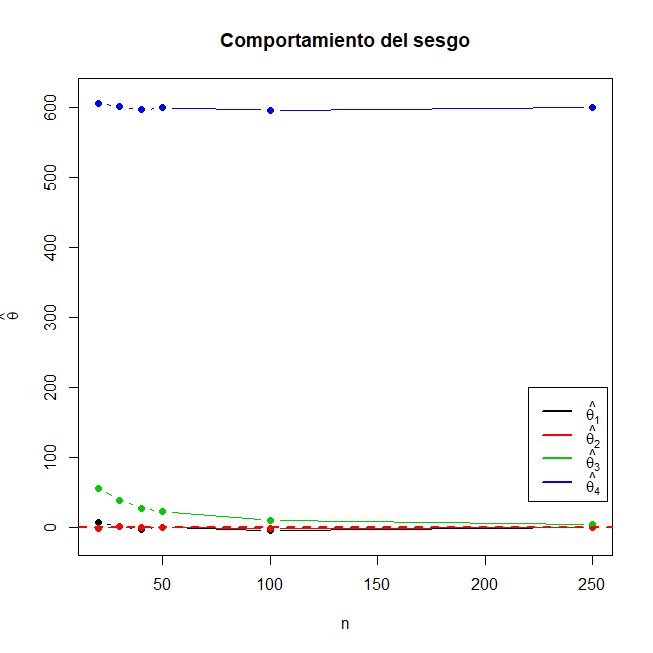
\includegraphics[width=10cm]{Figuras/S.png}
        \caption{Grafica del sesgo de los distintos estimadores variando los tama\~{n}os de muestra}
        \label{fig:Densidad}
    \end{center}
\end{figure}
~\\ En esta grafica vemos que al igual que en la anterior, los estimadores $\hat{\theta_1}$ y $\hat{\theta_2}$ son los mejores, ya que tienen un sesgo casi igual a 0 para todos los tama\~{n}os de muestra, aunque vemos tambien que el sesgo del estimador $\hat{\theta_3}$ tambien tiende a 0 a medida que se aumenta los tama\~{n}os de muestra. El estimador $\hat{\theta_4}$ es el menos acertado ya que su sesgo es muy elevado. En general, basandonos en esta grafica, los mejores estimadores hasta ahora son $\hat{\theta_1}$ y $\hat{\theta_2}$
\pagebreak \begin{figure}[!h]
    \begin{center}
        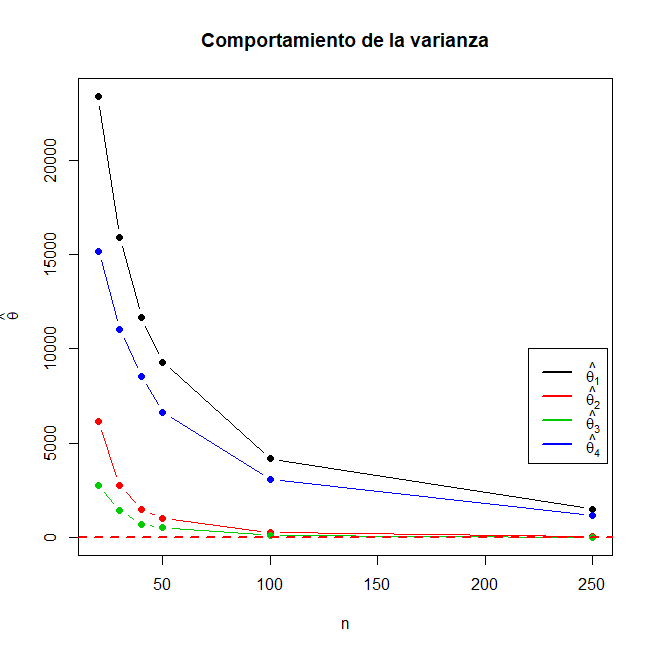
\includegraphics[width=10cm]{Figuras/V.png}
        \caption{Grafica de la varianza de los distintos estimadores variando los tama\~{n}os de muestra}
        \label{fig:Densidad}
    \end{center}
\end{figure}
~\\ En esta grafica podemos observar que los estimadores $\hat{\theta_2}$ y $\hat{\theta_3}$ tienen menor varianza que los otros dos, pero notemos, que la diferencia de varianzas entre $\hat{\theta_2}$ y $\hat{\theta_3}$ es casi la mitad a favor de $\hat{\theta_3}$ en los tama\~{n}os de muestra mas peque\~{n}os, indicandonos esto, que el estimador de menor varianza es efectivamente $\hat{\theta_3}$.
\pagebreak \begin{figure}[!h]
    \begin{center}
        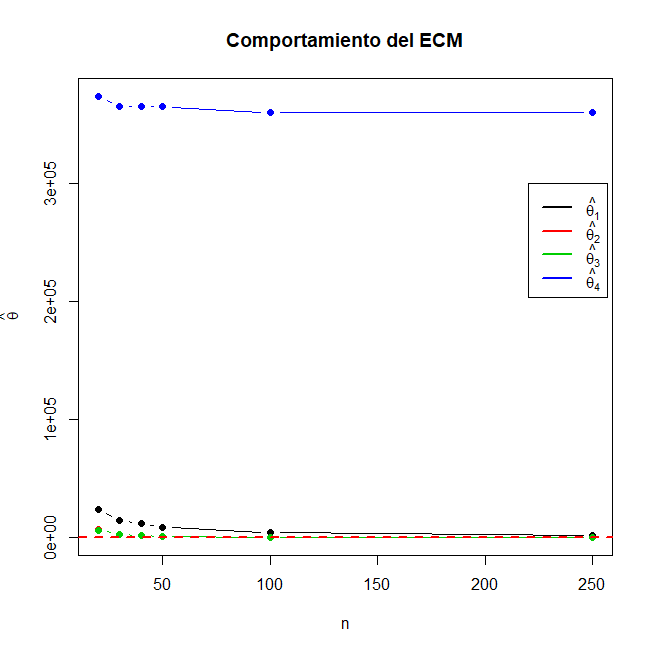
\includegraphics[width=10cm]{Figuras/ECM.png}
        \caption{Grafica del ECM de los distintos estimadores variando los tama\~{n}os de muestra}
        \label{fig:Densidad}
    \end{center}
\end{figure}
~\\ En la grafica anterior, notamos que el menor Error cuadratico medio lo presentan los estimadores $\hat{\theta_2}$ y $\hat{\theta_3}$, con casi el mismo en todos los tama\~{n}os de muestra, por esa razon no logramos ver la linea y los puntos que representan el estimador $\hat{\theta_2}$, pero en el tama\~{n}o de muestra n=5 se alcanza a observar una peque\~{n}a porcion del punto rojo que representa el estimador $\hat{\theta_2}$, obstruido por el punto verde que representa el estimador $\hat{\theta_3}$, lo que nos asegura que no hay diferencias significativas entre estos estimadores con respecto al ECM.Entonces, para decidir cual de los dos estimadores es mejor, debemos ver las 4 graficas en conjunto, ya que el ECM no me deja claro esto, por ser tan parecido en ambos.

~\\ En conclusion, tomando en cuenta las 4 graficas, podriamos decir que para tama\~{n}os de muestra menor a 100, $\hat{\theta_2}$ es el mejor estimador para $\theta=1200$ ya que su sesgo es menor que el de $\hat{\theta_3}$, su estimacion es mas cercana al valor real del parametro y ademas su varianza no es muy alta. 


\pagebreak \section{Situacion 2}
\subsection{Punto A.}
~\\\textbf{Si $\hat{\theta_1}$ y $\hat{\theta_2}$ son dos estimadores insesgados tales que:
~\\$$\hat{\theta_3}=a{\hat{\theta_1}}+(1-a){\hat{\theta_2}}$$}
~\\ Aplico Esperanza a ambos lados 
~\\ $E[\hat{\theta_3}] = E[a{\hat{\theta_1}}+(1-a){\hat{\theta_2}}]$
~\\ $E[\hat{\theta_3}] = E[a{\hat{\theta_1}}]+E[(1-a){\hat{\theta_2}}]$
~\\ $E[\hat{\theta_3}] = aE[{\hat{\theta_1}}]+(1-a)E[{\hat{\theta_2}}]$ \textbf{Con $\hat{\theta_1}$ y $\hat{\theta_2}$ estimadores insesgados}\
~\\ $E[\hat{\theta_3}] = a{\theta} + (1-a){\theta}$
~\\ $E[\hat{\theta_3}] = a{\theta} + {\theta} - a{\theta}$
~\\ $$E[\hat{\theta_3}]={\theta}$$

~\\\textbf{$\therefore \hat{\theta_3}$ Es un estimador insesgado.} 
 


\subsection{Punto B.} 

~\\\textbf{ El coeficiente de variacion de $\hat{\theta_3}$ es}
~\\
~\\ $$CV[\hat{\theta_3}]=\frac{\sqrt{Var[\hat{\theta_3}]}}{E[\hat{\theta_3}]}$$
~\\ Hallamos la $Var[\hat{\theta_3}]$
~\\ $Var[\hat{\theta_3}]=Var[a{\hat{\theta_1}}+(1-a){\hat{\theta_2}}]+2Cov[a{\hat{\theta_1}},(1-a){\hat{\theta_2}}]$,    ya que no sabemos si ${\hat{\theta_1}}$ y ${\hat{\theta_2}}$ son independientes
~\\ Entonces, distribuyendo la Varianza y por las propiedades de Covarianza:
~\\ $Var[\hat{\theta_3}]=Var[a{\hat{\theta_1}}]+Var[(1-a){\hat{\theta_2}}]+2a(1-a) Cov[{\hat{\theta_1}},{\hat{\theta_2}}]$
~\\ $Var[\hat{\theta_3}]=a^2Var[{\hat{\theta_1}}]+(1-a)^2Var[{\hat{\theta_2}}]+(2a-2a^2)Cov[{\hat{\theta_1}},{\hat{\theta_2}}]$
~\\
~\\\textbf{Como $Var[{\hat{\theta_1}}]=\sigma_1^2$ y $Var[{\hat{\theta_2}}]=\sigma_2^2$ entonces}

~\\ $Var[\hat{\theta_3}]=a^2[\sigma_1^2]+(1-a)^2[\sigma_2^2]+(2a-2a^2)Cov[{\hat{\theta_1}},{\hat{\theta_2}}]$
~\\ Sabemos que $Cov[{\hat{\theta_1}},{\hat{\theta_2}}]= E[{\hat{\theta_1}}{\hat{\theta_2}}]- E[{\hat{\theta_1}}]*E[{\hat{\theta_2}}]$, entonces:
~\\ Como $E[{\hat{\theta_1}}]={\theta}$ y $E[{\hat{\theta_2}}]={\theta}$ tenemos:
~\\ $Cov[{\hat{\theta_1}},{\hat{\theta_2}}]=E[{\hat{\theta_1}}{\hat{\theta_2}}]-{\theta^2}$, por tanto:
~\\ $Var[\hat{\theta_3}]=a^2[\sigma_1^2]+(1-2a+a^2)[\sigma_2^2]+(2a-2a^2)(E[{\hat{\theta_1}}{\hat{\theta_2}}]-{\theta^2})$
~\\ Como sabemos que $E[\hat{\theta_3}]={\theta}$

~\\$\therefore$ \textbf{El coeficiente de variacion para $\hat{\theta_3}$ es:}  
$$CV[\hat{\theta_3}]=\frac{\sqrt{a^2\sigma_1^2+(1-a)^2\sigma_2^2+(2a-2a^2)(E[{\hat{\theta_1}}{\hat{\theta_2}}]-{\theta^2})}}{{\theta}}$$

\subsection{Punto C.} 
~\\ Como en este punto sabemos que $\hat{\theta_1}$ y $\hat{\theta_2}$ son independientes, entonces la $Cov[{\hat{\theta_1}},{\hat{\theta_2}}]=0$ y por tanto:
~\\ $Var[\hat{\theta_3}]=Var[a{\hat{\theta_1}}+(1-a){\hat{\theta_2}}]$
~\\ Distribuyendo la varianza y aplicando sus propiedades, nos queda:
~\\ $Var[\hat{\theta_3}]=Var[a{\hat{\theta_1}}]+Var[(1-a){\hat{\theta_2}}]$ 
~\\ $Var[\hat{\theta_3}]=a^2Var[{\hat{\theta_1}}]+(1-a)^2Var[{\hat{\theta_2}}]$
~\\ $Var[\hat{\theta_3}]=a^2\sigma_1^2+(1-a)^2\sigma_2^2$ 
~\\ Note que $Var[\hat{\theta_3}]$ se convierte en una funcion que depende de a, ya que, $\sigma_1^2$ y $\sigma_2^2$ son conocidas, entonces, debemos encontrar a, que haga minima dicha funcion, en otras palabras, todo se reduce a encontrar el minimo de la funcion. Para ello procedemos de la siguiente manera:
~\\ 1. Encontramos la primera derivada de la funcion con respecto a la variable a:
~\\ $$f'(a)=2a\sigma_1^2 - 2(1-a)\sigma_2^2$$
~\\ 2. Igualamos el resultado de la primera derivada a 0 y despejamos la variable que nos interesa obtener, en este caso, despejamos a:
$$2a\sigma_1^2 - 2(1-a)\sigma_2^2=0$$
$$2a\sigma_1^2 - (2-2a)\sigma_2^2=0$$
$$2a\sigma_1^2 - 2\sigma_2^2 + 2a\sigma_2^2=0$$
$$2a\sigma_1^2  + 2a\sigma_2^2= 2\sigma_2^2$$
$$a(2\sigma_1^2+2\sigma_2^2)=2\sigma_2^2$$
$$a=\frac{2\sigma_2^2}{2\sigma_1^2+2\sigma_2^2}$$
~\\$\therefore${$a=\frac{\sigma_2^2}{\sigma_1^2+\sigma_2^2}$}
~\\ 3. Ahora, debemos encontrar la segunda derivada y ver si es positiva o negativa para saber si encontramos un minimo o un maximo:
~\\$$f^{\prime\prime}(a)=2\sigma_1^2+2\sigma_2^2 > 0$$
~\\ Como nos dio que la segunda derivada parcial es siempre positiva, concluimos que el a hallado anteriormente es un minimo. Por lo tanto, para hacer que la $Var[\hat{\theta_3}]$ sea minima, debemos escoger a como $a=\frac{\sigma_2^2}{\sigma_1^2+\sigma_2^2}$.

\section{Situacion 3}
\subsection{Punto A.}

Sea $X$ una distribucion Poisson$(\lambda)$ con, $n=30$ y $E[x]=(\lambda)$

$$\ M'_1 = \frac{1}{30} \sum_{i=1}^{30}x_{i}$$
$$\mu'_1 = \lambda$$

$\ M'_1 = \frac{1}{30} \sum_{i=1}^{30}x_{i} = \lambda = \mu'_1$

$\therefore \hat{\lambda}= \frac{1}{30} \sum_{i=1}^{30}x_{i} = \overline{X}$
 
~\\Ahora es necesario probrar si es insesgado: 

~\\$E[\hat{\lambda}]=E[\frac{1}{30} \sum_{i=1}^{30}x_{i}]$
~\\$E[\hat{\lambda}]=\frac{1}{30} E[\sum_{i=1}^{30}{\lambda}_{i}]$
~\\$E[\hat{\lambda}]=\frac{1}{30}30\lambda$
~\\$E[\hat{\lambda}]=\lambda$

~\\$\therefore$ \textbf{Un estimador insesgado para} $\lambda$ \textbf{es} $\hat{\lambda}= \frac{1}{30} \sum_{i=1}^{30}x_{i} = \overline{X}$

\subsection{Punto B.}

Sea $C=3X+X^2$

~\\$E[C]=E[3X+X^2]$
~\\$E[C]=E[3X] + E[X^2]$
~\\$E[C]=3E[X] + E[X^2]$

~\\ Sabiendo que:
 
$V[X]=E[X^2] - E^2[X]$


~\\ Entonces: 

$E^2[X] = V[X] + E[X^2]$

~\\$\therefore E^2[X] = \lambda + (\lambda)^2$

~\\ Reemplazando $E^2[X]$ en:\ 

$E[C]=3\lambda + E[X^2]$

~\\Obtenemos que: 
$E[C]=3\lambda + \lambda + (\lambda)^2$
~\\$\therefore E[C] = 4\lambda + (\lambda)^2$

\section{Situacion 5}
\subsection{Punto A.}
~\\ Tenemos la siguiente informacion del problema:
~\\ $\mu=3800$  $\sigma=400psi$ $n=4$ y $\bar{X}=3334$ el cual es el valor de la media sobre la cual se toma la decision.
~\\ Para responder a la pregunta sobre el riesgo que corre el proveedor bajo este criterio de decision, decidimos calcular la probabilidad de que $\bar{X}\leq3334$, entonces:
~\\ Sabemos que $\bar{X}\sim{N(\mu_x,\frac{\sigma}{\sqrt{n}}})$, en este caso $\bar{X}\sim{N(\mu_x=3800,\frac{\sigma=400}{\sqrt{4}}})=(\mu_x=3800,\sigma=200)$
~\\Entonces:
~\\ $P(\bar{X}\leq3334)=P(Z\leq\frac{3334-3800}{200})=P(Z\leq\frac{-466}{200})=P(Z\leq-2.33)=0.0099$ (Utilizando la tabla de la normal estandar)
~\\Segun lo anterior, logramos ver que la probabilidad de que la media sea menor que 3344 es tan solo de 0.99\%, entonces concluimos que el riesgo que corre el proveedor de que el cliente les devuelva un lote bajo esta regla de decision es muy bajo, de hecho, segun los resultados, de cada 100 lotes, solo le devolvera uno aproximadamente. El riesgo lo corre mas bien el comprador, ya que este, con la regla de decision establecida no va a lograr concluir casi nunca que el proceso esta fuera de control cuando en realidad lo esta. Por ultimo, viendolo en forma de errores tipo 1 y 2, concluimos que esta regla de decision cuenta con una probabilidad de cometer error tipo 2 muy alta, es decir, la mayoria de veces va a concluir que el proceso esta bajo control, cuando en realidad esta fuera de control.
\subsection{Punto B.}
~\\ Si se cambia la media a $\mu=3700$, la probabilidad que existe de que un lote sea detectado bajo estas condiciones es la siguiente:
~\\ $P(\bar{X}\leq3334)=P(Z\leq\frac{3334-3700}{200})=P(Z\leq\frac{-366}{200})=P(Z\leq-1.83)=0.0336$ (Utilizando la tabla de la normal estandar)
~\\ Con lo anterior, podemos observar que la probabilidad de que un lote sea detectado bajo esas condiciones es de 3.36\%, un poco mas alto que en el punto anterior, esto nos dice que entre mas cerca este $\mu$ del valor de la media muestral $\bar{X}$, mas alta va a ser esta probabilidad, y por consiguiente, las posibilidades de que el cliente detecte el lote van a ser mayores.
\pagebreak \subsection{Punto C.}
\begin{figure}[!h]
    \begin{center}
        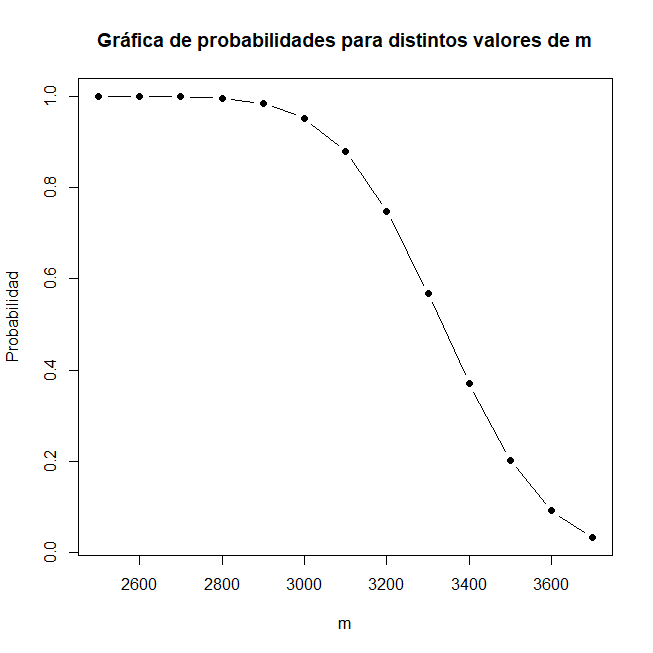
\includegraphics[width=10cm]{Figuras/5.png}
        \caption{Grafica de probabilidades de detectar el lote segun la media $\mu$}
        \label{fig:Densidad}
    \end{center}
\end{figure}
~\\ En esta grafica podemos ver que mientras el valor de la media $\mu$ aumenta, la probabilidad de detectar el lote va disminuyendo, esto pasa, porque la resistencia media con la cual se dice que el proceso de produccion esta bajo control es de 3800 psi, entonces a medida que la media muestral aumenta, nos vamos acercando mas a la media teorica (3800 en este caso), lo que hace menos probable que se devuelva un lote de varillas metalicas, ya que mientras mas cercana sea la media muestral a la poblacional, tenemos mas certeza para concluir que las varillas se estan haciendo con el proceso adecuado o bajo control.
% Bibliografia utilizada 
\bibliography{Bibliografia}
\end{document}